\section{Java Sample applications}
\label{sec:JavaSampleApps}

The first two examples in this section are simple applications developed in COMPSs to easily illustrate how to code,
compile and run COMPSs applications. These applications are executed locally and show different ways to take advantge
of all the COMPSs features. 

The rest of the examples are more elaborated and consider the execution in a cloud platform where the VMs mount a common 
storage on \textbf{/sharedDisk} directory. This is useful in the case of applications that require working 
with big files, allowing to transfer data only once, at the beginning of the execution, and to enable 
the application to access the data directly during the rest of the execution.

The Virtual Machine available at our webpage (\url{http://compss.bsc.es/}) provides a development environment with
all the applications listed in the following sections. The codes of all the applications can be found under the 
$/home/compss/workspace\_java/$ folder. 

%%%%%%%%%%%%%%%
%% HELLO WORLD 
%%%%%%%%%%%%%%%
\subsection{Hello World}


%%%%%%%%%%%%%%%
%% SIMPLE
%%%%%%%%%%%%%%%
\subsection{Simple}


%%%%%%%%%%%%%%%
%% Increment
%%%%%%%%%%%%%%%
\subsection{Increment}


%%%%%%%%%%%%%%%
%% MATMUL
%%%%%%%%%%%%%%%
\subsection{Matrix multiplication}
Matrix Multiplication (Matmul) is a pure Java application that multiplies two matrices in a direct way. 
The application creates 2 matrices of N x N size initialized with values, and multiply the matrices by 
blocks of 40 floats (by default).

\begin{figure}[ht!]
  \centering
    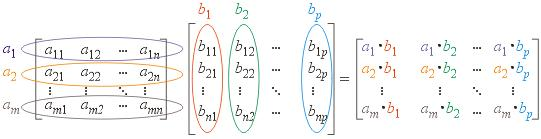
\includegraphics[width=0.8\textwidth]{./Sections/2_Java/Figures/matrix.jpeg}
    \caption{Matrix multiplication} 
    \label{fig:matrix}
\end{figure}

In this application the multiplication is implemented in the multiplyAccumulative that is thus selected 
as the task that will be executed remotely. In order to run the application the matrix dimension has to 
be supplied.

\begin{lstlisting}[language=bash]
compss@bsc:~$ cp ~/workspace_java/matmul/package/Matmul.tar.gz /home/compss/
compss@bsc:~$ tar xzf Matmul.tar.gz
\end{lstlisting}

The command line to execute the application:

\begin{lstlisting}[language=bash]
compss@bsc:~$ runcompss matmul.Matmul <matrix_dim>
\end{lstlisting}

%%%%%%%%%%%%%%%
%% SPARSELU 
%%%%%%%%%%%%%%%
\subsection{Sparse LU decomposition}
SparseLU multiplies two matrices using the factorization method of LU decomposition, which factorizes a 
matrix as a product of a lower triangular matrix and an upper one.

\begin{figure}[ht!]
  \centering
    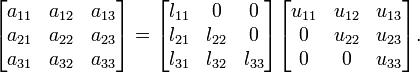
\includegraphics[width=0.6\textwidth]{./Sections/2_Java/Figures/SparseLU.jpeg}
    \caption{Sparse LU decomposition}
    \label{fig:SparseLO}
\end{figure}

The matrix is divided into N x N blocks on where 4 types of operations will be applied modifying the blocks: 
{\bf lu0}, {\bf fwd}, {\bf bdiv} and {\bf bmod}. These four operations are implemented in four methods that 
are selecetd as the tasks that will be executed remotely. In order to run the application the matrix dimension 
has to be provided.

\begin{lstlisting}[language=bash]
compss@bsc:~$ cp ~/workspace/sparselu/package/SparseLU.tar.gz /home/compss/
compss@bsc:~$ tar xzf SparseLU.tar.gz
\end{lstlisting}

The command line to execute the application:

\begin{lstlisting}[language=bash]
compss@bsc:~$ runcompss sparselu.SparseLU <matrix_dim>
\end{lstlisting}


%%%%%%%%%%%%%%%
%% KMEANS
%%%%%%%%%%%%%%%
\subsection{KMeans}


%%%%%%%%%%%%%%%
%% BLAST
%%%%%%%%%%%%%%%
\subsection{BLAST Workflow}
BLAST is a widely-used bioinformatics tool for comparing primary biological sequence information, such as 
the amino-acid sequences of different proteins or the nucleotides of DNA sequences with sequence databases, 
identifying sequences that resemble the query sequence above a certain threshold. 
The work performed by the COMPSs Blast workflow is computationally intensive and embarrassingly parallel.

\begin{figure}[ht!]
  \centering
    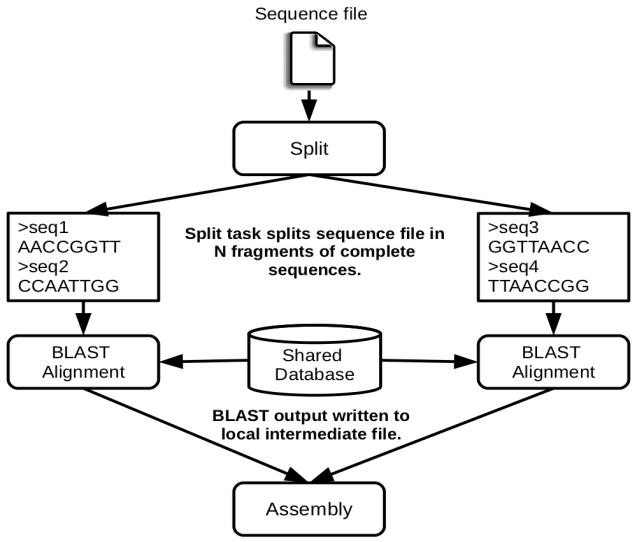
\includegraphics[width=0.7\textwidth]{./Sections/2_Java/Figures/blast_workflow.jpeg}
    \caption{The COMPSs Blast workflow}
    \label{fig:BLAST_workflow}
\end{figure}

The workflow describes the three blocks of the workflow implemented in the {\bf Split}, {\bf Align} and 
{\bf Assembly} methods. The second one is the only method that is chosen to be executed remotely, so it 
is the unique method defined in the interface file. The {\bf Split} method chops the query sequences file 
in N fragments, {\bf Align} compares each sequence fragment against the database by means of the Blast 
binary, and {\bf Assembly} combines all intermediate files into a single result file.

This application uses a database that will be on the shared disk space avoiding transferring the entire 
database (which can be large) between the virtual machines.

\begin{lstlisting}[language=bash]
compss@bsc:~$ cp ~/workspace/blast/package/Blast.tar.gz /home/compss/
compss@bsc:~$ tar xzf Blast.tar.gz
\end{lstlisting}

The command line to execute the workflow:

\begin{lstlisting}[language=bash]
compss@bsc:~$ runcompss blast.Blast <debug> 
                                    <bin_location>
                                    <database_file> 
                                    <sequences_file>
                                    <frag_number> 
                                    <tmpdir>
                                    <output_file>
\end{lstlisting}

Where:
\begin{itemize}
 \item {\bf debug}: The debug flag of the application (true or false).
 \item {\bf bin\_location}: Path of the Blast binary.
 \item {\bf database\_file}: Path of database file; the shared disk {\bf /sharedDisk/} is suggested to avoid big data transfers.
 \item {\bf sequences\_file}: Path of sequences file.
 \item {\bf frag\_number}: Number of fragments of the original sequence file, this number determines the number of parallel Align tasks.
 \item {\bf tmpdir}: Temporary directory ({\bf /home/compss/tmp/}).
 \item {\bf output\_file}: Path of the result file.
\end{itemize}
 
Example:
\begin{lstlisting}[language=bash]
compss@bsc:~$ runcompss blast.Blast true
                        /home/compss/workspace_java/blast/binary/blastall
                        /sharedDisk/Blast/databases/swissprot/swissprot
                        /sharedDisk/Blast/sequences/sargasso_test.fasta 
                        4 
                        /tmp/
                        /home/compss/out.txt
\end{lstlisting}